\subsection{Elettrodo di prima specie}
Gli elettrodi visti finora appartengono a questa categoria. Essi sono metalli immersi in soluzioni dei loro ioni. Si fa ciò per raggiungere molto più velocemente l'equilibrio tra soluzione ed elettrodo, in quanto in acqua l'equilibrio è molto lento perché turbato dalla presenza degli ioni $\rm H_3O^+$ che competono assieme agli ioni liberati dal metallo nell'acqua per ritornare sull'elettrodo stesso.

L'elettrodo partecipa attivamente alla reazione, ossia è il metallo che libera ioni in soluzione, i quali lasciano elettroni sul metallo:

$$\ce{M <--> M^{n+} + ne^-}$$

$$\ce{AgCl(s) <--> Ag^+ + Cl^-}$$

$$\ce{Ag^+ e^- <--> Ag}$$

$$\ce{AgCl(s) + e^- <--> Ag + Cl^-}$$
\subsection{Elettrodo di seconda specie}
In questo caso il metallo è a contatto con un suo sale poco solubile, ad esempio argento Ag a contatto con cloruro di argento AgCl che è un sale insolubile. A sua volta il sale è a contatto con una soluzione di un sale (ovviamente solubile) che abbia l'anione in comune col sale poco solubile, quindi nel nostro esempio dovrà essere un sale che ha come anione ha lo ione cloruro, come il cloruro di potassio KCl
\subsection{Elettrodo di terza specie}

Scriviamo le equazioni di Nernst relative ai vari elettrodi:

\vspace{0.2cm} $\bullet$\textbf{Elettrodo di prima specie}

$$\ce{Cu^{2+} + 2e^- <--> Cu} \quad E= E_0 + \frac{0.059}{2}\log \frac{a_{\text{Cu}^{2+}}}{a_{\text{Cu}}}$$

$$a_{\text{Cu}}=1 \implies E= E_0 + \frac{0.059}{2}\log a_{\text{Cu}^{2+}}$$

Questa sarà la d.d.p. di questo semielemento/elettrodo.

Va da ricordare che poi nei calcoli usiamo la concentrazione, non l'attività.

\vspace{0.2cm} $\bullet$\textbf{Elettrodo di terza specie}

Per convenzione le reazioni si scrivono come riduzione, quindi

$$\rm Pt\,/\,Fe^{2+}, \; Fe^{3+} \implies \ce{Fe^{3+} + e^- <--> Fe^{2+}} $$

$$E = E_0 + \frac{0.059}{1} \log \frac{a_{\text{Fe}^{3+}}}{a_{\text{Fe}^{2+}}}$$

$$\rm Pt\,/\,Mn^{2+}, \; MnO_4^- \implies \ce{MnO_4^- + 8H^+ + 5e^- <--> Mn^{2+} + 4H_2O} $$

$$E = E_0 + \frac{0.059}{5} \log \frac{a_{\text{MnO}_4^-} \cdot a^8_{\text{H}^+}}{a_{\text{Mn}^{2+}}}$$
\subsection{Elettrodo normale standard ad idrogeno}
Finora non siamo stati in grado di misurare i potenziali. Per fare ciò si sceglie un elettrodo e si usa come riferimento. Ad esso si assegna un potenziale arbitrario (nel caso particolare si è assegnato valore zero) e si usa questo come secondo elettrodo per fare le misure di tutti i potenziali di qualunque altro elettrodo.

Quindi la d.d.p. tra elettrodo e soluzione non è misurabile perché dovremmo introdurre un tester che farebbe da secondo elettrodo. Allora si è scelto l'elettrodo normale standard a idrogeno

\begin{minipage}{0.55\textwidth}
    \begin{figure}[H]
        \centering
        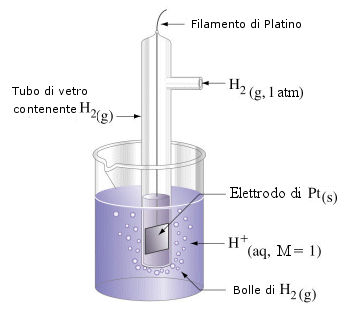
\includegraphics[width=8cm]{immagini/Elettrodo_a_idrogeno.png}
    \end{figure}
\end{minipage}
\begin{minipage}{0.45\textwidth}
    Immaginiamo di avere un beker contenente una soluzione 1-molare di HCl in cui mettiamo un filo di platino saldato ad una lamina di platino, la quale in superficie è ricoperta di una polvere finissima di platino. Tale oggetto si chiama \textit{platino platinato}. Viene rivestito per aumentare la superficie di disposizione, perché si conta la superficie di ogni granello.
\end{minipage}

\subsection{Elettrodo a calomelano saturo}
\E un elettrodo a mercurio ed è quello che poi viene usato nella pratica. Si chiama così perché è presente il composto $\rm Hg_2Cl_2$, che si chiama calomelano.

Perché non possiamo semplificare i pedici in $\rm Hg_2Cl_2$?

Perché lo ione in soluzione non è $\rm Hg^+$ ma è $\rm Hg_2^{2+}$, cioè ci sono due ioni che stanno assieme formando un dimero.

\begin{minipage}{0.35\textwidth}
    \begin{figure}[H]
        \centering
        \includegraphics[width=5cm]{immagini/Elettrodo_a_calomelano.png}
    \end{figure}
\end{minipage}
\begin{minipage}{0.63\textwidth}
    \vspace{0.4cm}Tale elettrodo è costituito da un bulbo di vetroin cui abbiamo mercurio Hg liquido. Per realizzare il contatto elettrico è saldato al bulbo un filo di platino che tocca il mercurio dentro ed esce fuori. In questo modo il contatto elettrico è assicurato sia dentro che fuori.

    Il metallo deve essere a contatto con una soluzione di un suo sale poco solubile, che è l'$\rm Hg_2Cl_2$. Questo a sua volta è a contatto con un sale con cui ha in comune l'anione, che è il KCl. Quest'ultimo si trova nella gelatina di agar-agar che costituisce il ponte salino. In questo modo in questo elettrodo abbiamo entrambi i collegamenti: il filo metallico e il ponte salino per collegarlo ad un'altra soluzione.
\end{minipage}

\vspace{0.2cm}Ciò che avviene è che l'$\rm Hg_2Cl_2$ si dissocia in $\rm Hg_2^{2+}$ più due ioni cloruro $\rm Cl^-$:

$$\ce{Hg_2Cl_2(s) <--> Hg_2^{2+} + 2Cl^-}$$

Se poi ad $\rm Hg_2^{2+}$ forniamo due elettroni otteniamo due atomi di mercurio:

$$\ce{ Hg_2^{2+} + 2e^- <--> 2Hg}$$

Globalmente la reazione sarà

$$\ce{Hg_2Cl_2(s) + 2e^- <--> 2Hg + 2Cl^-}$$

Il potenziale di questa reazione sarà

$$E=E_0 + \frac{0.059}{2} \log \frac{a_{\text{Hg}_2\text{Cl}_2(s)}}{a^2_{\text{Hg}} \cdot a^2_{\text{Cl}^-}}$$

Il mercurio è un metallo puro, quindi la sua attività è unitaria. Il calomelano saturo è un solido puro e l'attività dei solidi è sempre unitaria. Quindi resta

$$E=E_0 + \frac{0.059}{2} \log \frac{1}{a^2_{\text{Cl}^-}}\quad
\implies E=E_0 + \frac{0.059}{2} \log a^{-2}_{\text{Cl}^-}$$

$$\implies E=E_0 - \frac{0.059}{2} \cdot 2 \log a_{\text{Cl}^-}
\quad
\implies E=E_0 - 0.059 \log a_{\text{Cl}^-}$$

Il potenziale di Nerst di questo elettrodo dipenderà allora dalla concentrazione dello ione cloruro (infatti se misuriamo una d.d.p. tra questo elettrodo e quello nromale standar a idrogeno, dato che per definzione il potenziale del secondo è pari a zero, quello che misuriamo è imputabile tutto a questo elettrodo). Abbiamo così scoperto un modo per misurare la concentrazione di uno ione.
\subsection{Elettrodo d'argento}
$$\ce{AgCl + 1e^- <--> Ag + Cl^-}$$
Il potenziale sarà
$$E = E_0 -0.059 \log a_{\text{Cl}^-}$$
\subsection{Elettrodo al chinidrone}
\begin{center}
    \begin{tabular}{p{2.4cm}p{2.5cm}p{2.1cm}p{2cm}}
    \chemfig{*6(-(=O)-=-(=O)-=)} & \vspace{-0.8cm}$\rm + \; 2H^+ \; + \; 2e^-$ & \vspace{-0.9cm} \schemestart \arrow{<=>}      \schemestop &
    \chemfig{*6(=(-OH)-=-(-OH)=-)}\\
    \vspace{0.2cm}\hspace{-0.1cm}Benzochinone & & & \vspace{0.2cm}Idrochinone
    \end{tabular}
\end{center}

Il potenziale sarà

$$E = E_0 + \frac{0.059}{2} \log \frac{a_{\text{Benzochinone}} \cdot a^2_{\text{H}^+}}{a_{\text{Idrochinone}}}$$

$$E = E_0 + 0.059 \log a_{\text{H}^+}$$

$$E = E_0 - 0.059 \log \left( \frac{1}{a_{\text{H}^+}} \right)$$

\subsubsection{Excursus: la placcatura}
Placcare qualcosa in un certo metallo significa avere una solzione di questo in cui immergiamo l'oggetto che vogliamo ricoprire e alla quale applichiamo una d.d.p. in modo tale che il metallo si depositi come un film sottile omogeneo.

Quali metalli possiamo far depositare in acqua? Tutti quelli che hanno il potenziali maggiore di zero, perché altrimenti anziché ridursi il metallo gli elettroni saranno presi dall'idrogeno piuttosto che dagli ioni metallici.

Quindi si riducono le speci che hanno il potenziale standard maggiore. Tutti gli elementi a potenziale negativo non vedranno mai sviluppata la loro riduzione in soluzione, al loro posto sarà lo ione $\rm H^+$ a ridursi in idrogeno: \ce{2H^+ <--> H_2}.

\begin{center}
    \scriptsize\begin{tabular}{|ll|ll|}
        \hline
        &&&\\
        Reazione & $E_0 \; (V)$ & Reazione & $E_0 \; (V)$\\
        &&&\\
        \hline
        &&&\\
        \ce{Li^+ + e^- <--> Li} & -3.045 & \ce{S_4O_6^{2-} <--> 2S_2O_3^{2-}} & 0.10\\[0.7ex]
        \ce{K^+ + e^- <--> K} & -3.924 & \ce{S + 2H_3O^+ + 2e^- <--> H_2S + 2H_2O} & 0.14\\[0.7ex]
        \ce{Ca^{2+} + 2e <--> Ca} & -2.76 & \ce{Sn^{4+} 2e^- <--> Sn^{2+} (HCl \; 1F)} & 0.15\\[0.7ex]
        \ce{Na^+ + e^- <--> Na} & -2.7109 & \ce{Cu^{2+} + e^- <--> Cu^+} & 0.158\\[0.7ex]
        \ce{Mg^{2+} + 2e^- <--> Mg} & -2.375 & \ce{Hg_2Cl_2 + 2e^- <--> 2Hg + 2Cl^-} & 0.2682\\[0.7ex]
        \ce{H_3O^+ + e^- <--> H_2O + H} & -2.10 & \ce{Cu^{2+} + 2e^- <--> Cu} & 0.337\\[0.7ex]
        \ce{Al^{3+} + 3e^- <--> Al} & -1.71 & \ce{O_2 + 2H_2O + 4e^- <--> 4OH^-} & 0.401\\[0.7ex]
        \ce{} & & \ce{} & \\[0.7ex]
        \ce{} & & \ce{} & \\[0.7ex]
        \ce{} & & \ce{} & \\[0.7ex]
        \ce{} & & \ce{} & \\[0.7ex]
        \ce{} & & \ce{} & \\[0.7ex]
        \ce{} & & \ce{} & \\[0.7ex]
        \ce{} & & \ce{} & \\[0.7ex]
        \ce{} & & \ce{} & \\[0.7ex]
        \ce{} & & \ce{} & \\[0.7ex]
        \ce{} & & \ce{} & \\[0.7ex]
        \ce{} & & \ce{} & \\[0.7ex]
        \ce{} & & \ce{} & \\[0.7ex]
        \ce{} & & \ce{} & \\[0.7ex]
        \ce{} & & \ce{} & \\[0.7ex]
        \ce{} & & \ce{} & \\[0.7ex]
        \ce{} & & \ce{} & \\[0.7ex]
        \ce{} & & \ce{} & \\[0.7ex]
        \ce{} & & \ce{} & \\[0.7ex]
        \ce{} & & \ce{} & \\[0.7ex]
        \ce{Pb + 2e^- <--> Pb} & -0.1263 & \ce{H_2O_2 + 2H_3O^+ + 2e^- <--> 4H_2O} & 1.776\\[0.7ex]
        \ce{2H_3O^+ + 2e^- <--> H_2 + 2H_2O} & 0.000 & \ce{Co^{3+} + e^- <--> Co^{2+} (HNO_3 \; 3F)} & 1.842\\[0.7ex]
        \ce{NO_3^- + H_2O + 2e^- <--> NO_2^- + 2OH^-} & 0.0 & \ce{F_2 + 2e <--> 2F^-} & 2.87\\[0.7ex]
        \hline
    \end{tabular}
\end{center}
\normalsize